%% 4.3 Building a Datapath
%% Included from mips.tex via \input

\section{Datapath Elements}

A datapath is the collection of state elements, computation units, and
interconnections that together perform the data processing operations
required by the instruction set.

\subsection{Instruction Fetch}

The first step in executing any instruction is to fetch it from memory.
This requires two state elements and an adder:

\begin{itemize}
  \item \textbf{Instruction memory} --- stores the program's instructions
        and supplies the instruction specified by an address.
  \item \textbf{Program counter (PC)} --- a register that holds the address
        of the current instruction.
  \item \textbf{Adder} --- computes the next instruction address by adding
        4 (the size of one instruction) to the current PC value.
\end{itemize}

\begin{figure}[htbp]
  \centering
  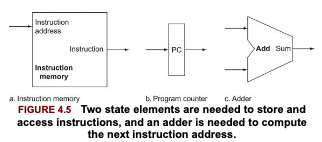
\includegraphics[width=0.7\textwidth]{figures/figure_4.5.png}
  \label{fig:4.5}
\end{figure}

\section{Lisp Tips}

\subsection{Defining Functions}

Use \texttt{defun} to define a named function.
The general form is:

\begin{lstlisting}
(defun function-name (param1 param2 ...)
  body)
\end{lstlisting}

A function that takes two arguments and adds them:

\begin{lstlisting}
(defun add (a b)
  (+ a b))

(add 3 5)  ; => 8
\end{lstlisting}

\subsection{Binary and Hexadecimal Literals}

Common Lisp supports number literals in any base:

\begin{lstlisting}
#b1010      ; binary      => 10
#o17        ; octal        => 15
#xFF        ; hexadecimal  => 255
\end{lstlisting}

To print a number in binary:

\begin{lstlisting}
(format t "~B~%" 42)   ; => 101010
\end{lstlisting}

\subsection{Reading Files with \texttt{with-open-file}}

\texttt{with-open-file} opens a file, binds it to a stream variable,
and automatically closes it when the body finishes.

\begin{lstlisting}
(with-open-file (stream "path/to/file"
                        :direction :input)
  ;; use stream here
  )
\end{lstlisting}

The \texttt{:direction} keyword controls the mode.
It defaults to \texttt{:input}, so it can be omitted when reading.

\begin{center}
\begin{tabular}{lll}
  \toprule
  \textbf{Direction} & \textbf{Description} & \textbf{Required?} \\
  \midrule
  \texttt{:input}  & Read from file & No (default) \\
  \texttt{:output} & Write to file  & Yes \\
  \bottomrule
\end{tabular}
\end{center}

Read a single value (number or S-expression):

\begin{lstlisting}
(with-open-file (s "data.txt")
  (read s))
\end{lstlisting}

Read one line as a string:

\begin{lstlisting}
(with-open-file (s "data.txt")
  (read-line s))
\end{lstlisting}

Write to a file:

\begin{lstlisting}
(with-open-file (s "out.txt" :direction :output)
  (format s "Hello~%"))
\end{lstlisting}

\subsection{The \texttt{loop} Macro}

\texttt{loop} is Common Lisp's general-purpose iteration construct.
Unlike most Lisp forms, \texttt{loop} uses English-like \textbf{clauses}
instead of nested parentheses. A loop is built by chaining clauses together:

\begin{lstlisting}
(loop <clause-1>
      <clause-2>
      ...)
\end{lstlisting}

\subsubsection{Clause Reference}

\begin{center}
\begin{tabular}{lllp{5.5cm}}
  \toprule
  \textbf{Category} & \textbf{Required?} & \textbf{Clause} & \textbf{Meaning} \\
  \midrule
  Variable      & Yes & \texttt{for x from a to b}   & Count from \texttt{a} to \texttt{b} \\
                &     & \texttt{for x in list}        & Bind \texttt{x} to each element of \texttt{list} \\
                &     & \texttt{for x = expr}         & Re-evaluate \texttt{expr} every iteration \\
  \midrule
  Init          & No  & \texttt{with x = expr}        & Initialize \texttt{x} once before the loop starts \\
  \midrule
  Termination   & No  & \texttt{while test}           & Continue while \texttt{test} is true \\
                &     & \texttt{until test}           & Stop when \texttt{test} becomes true \\
  \midrule
  Body / Action & Yes & \texttt{do (expr)}            & Execute \texttt{expr} as a side-effect \\
                &     & \texttt{collect expr}         & Gather results into a list \\
                &     & \texttt{sum expr}             & Accumulate a running total \\
  \bottomrule
\end{tabular}
\end{center}

Variable and Body each require at least one clause.
Pick whichever fits your use case from the options listed.

\subsubsection{Execution Order}

Each iteration of the loop proceeds in this order:

\begin{enumerate}
  \item \textbf{Step} --- update all \texttt{for} variables
        (\texttt{from}/\texttt{in}/\texttt{=}).
  \item \textbf{Test} --- check \texttt{while}/\texttt{until}; exit if
        the condition fails.
  \item \textbf{Body} --- execute \texttt{do}, \texttt{collect},
        \texttt{sum}, etc.
  \item Go back to step 1.
\end{enumerate}

\subsubsection{Examples}

\paragraph{Simple counting.}

\begin{lstlisting}
(loop for i from 0 below 5
      do (format t "~A~%" i))
;; prints 0 through 4
\end{lstlisting}

Breakdown: \texttt{for i from 0 below 5} sets \texttt{i} to 0, 1, 2,
3, 4. \texttt{below} means exclusive (\texttt{to} is inclusive).

\paragraph{Iterating over a list.}

\begin{lstlisting}
(loop for x in '(10 20 30)
      do (format t "~A~%" x))
\end{lstlisting}

\texttt{for x in list} binds \texttt{x} to the next element each
iteration. The loop ends when the list is exhausted.

\paragraph{Collecting results into a list.}

\begin{lstlisting}
(loop for i from 1 to 5
      collect (* i i))
; => (1 4 9 16 25)
\end{lstlisting}

\texttt{collect} gathers each value and returns the whole list when the
loop finishes.

\paragraph{Reading lines from a stream until EOF.}

\begin{lstlisting}
(with-open-file (s "input.txt")
  (loop for line = (read-line s nil)
        while line
        do (format t "~A~%" line)))
\end{lstlisting}

\begin{itemize}
  \item \texttt{for line = (read-line s nil)} --- re-evaluate
        \texttt{read-line} every iteration.
        The second argument \texttt{nil} means return \texttt{nil}
        at EOF instead of signaling an error.
  \item \texttt{while line} --- stop when \texttt{line} is \texttt{nil}.
  \item \texttt{do ...} --- execute the body.
\end{itemize}

\paragraph{Multiple clauses combined.}

\begin{lstlisting}
(loop with total = 0
      for i from 1 to 10
      do (setf total (+ total i))
      finally (format t "Sum: ~A~%" total))
; => Sum: 55
\end{lstlisting}

\texttt{with total = 0} initializes once.
\texttt{finally} runs after the loop ends.

\subsection{Assignment: \texttt{setf} vs \texttt{loop}'s \texttt{=}}

These serve different purposes depending on context.

\paragraph{Inside \texttt{loop}: use \texttt{for x = expr}.}
This is part of the \texttt{loop} syntax. The expression is
re-evaluated on every iteration.

\begin{lstlisting}
(loop for line = (read-line s nil)
      while line
      do (format t "~A~%" line))
\end{lstlisting}

\paragraph{Outside \texttt{loop}: use \texttt{setf}.}
\texttt{setf} is the general assignment operator for variables,
array elements, struct slots, etc.

\begin{lstlisting}
(defvar *pc* 0)
(setf *pc* (+ *pc* 4))  ; *pc* is now 4
\end{lstlisting}
